%--------------------------------------------------------------------------------
%\documentclass{article}

\documentclass[a4paper, 12pt]{article}
\usepackage[T1]{fontenc} 
\usepackage[bf]{caption}
\usepackage{hyperref}
\usepackage[all]{hypcap}
\usepackage[utf8]{inputenc}
\usepackage{graphicx}
\usepackage[czech, english]{babel}
\selectlanguage{czech}
\usepackage{subfig}                % \subfloat
\usepackage{color}
\usepackage{url}
\inputencoding{utf8}
%\usepackage[bf]{caption2}
\usepackage{hyperref}
\usepackage[all]{hypcap}
\hypersetup{colorlinks=false, linkbordercolor=1 1 1, citebordercolor=1 1 1}
\usepackage[right]{lineno}
\renewcommand\linenumberfont{\normalfont\tiny\color{blue}}


\title{Vykreslování sledováním paprsku s antialiasingem}
\author{Jan Wozniak <xwozni00@stud.fit.vutbr.cz>}
\date{\today}


%--------------------------------------------------------------------------------


\begin{document}
\selectlanguage{czech}
\maketitle

\section{Úvod}

Úkolem projektu bylo vytvořit jednoduchý raytracer v libovolném programovacím jazyku využívající tři metody pro odstranění aliasu.
Pro implementaci jsem zvolil jazyk Haskell, antialiasingové metody nadvzorkování, mip mapy a bilinearní interpolace.


%%%%%%%%%%%%%%%%%%%%%%%%%%%%%%%%%%%%%%%%%%%%%%%%%%%%%%%%%%%%%%%%%%%%%%%%%%%%%%%%%%%%%%%%

\section{Teorie}

\textit{Raytracing} je renderovací metoda jak z 3D scény udělat realistické 2D zobrazení. Rekurzivní princip kdy jsou z kamery vysílány paprsky
přes zobrazovací plátno do scény s modely objektů. 
Na obrázku \ref{fig:raytrace} je znázorněno, jak tento princip funguje.
V základní implementaci se dělí paprsky do tří skupin
\begin{itemize}
\item pohledový -- z kamery do scény
\item odražený -- z objektu sceny do objektu scény
\item stínový -- z objektu scény ke světlu
\end{itemize}

Pro výpočet průsečíku paprsků s jednoduššími objekty je možno použít základní rovnice analytické geometrie a vektorové algebry, které 
jsou k dispozici například v dokumentu Vector Algebra for Ray Tracing \cite{vectoralgerba}.

Při použití textur může docházet v obraze k nežádoucímu efektu zvanému \textit{aliasing}. 
V případě, že objekt má texturu obsahující příliš častou změnu barev, 
a objekt je ve velké vzdálenosti kde paprsky nevzorkují povrch objektu dostatečně často, jeví
se pozorovateli textura velmi zkresleně. Pro zmírnění tohoto efektu lze použít mimo jiné použít
\begin{itemize}
\item mip mapy -- několik textur s ruzným rozlišením v jediné textuře
\item supersampling -- nadvzorkování pixelu posíláním paprsků v rozích pixelu
\item bilinearní interpolaci -- nalezení přibližné hodnoty barvy ve spojitém prostoru z diskrétní textury
\end{itemize}


%\begin{equation}
%  \label{moje-rovnice}
%  c = a + b
%\end{equation}


\begin{figure}[htb]
  \centering
  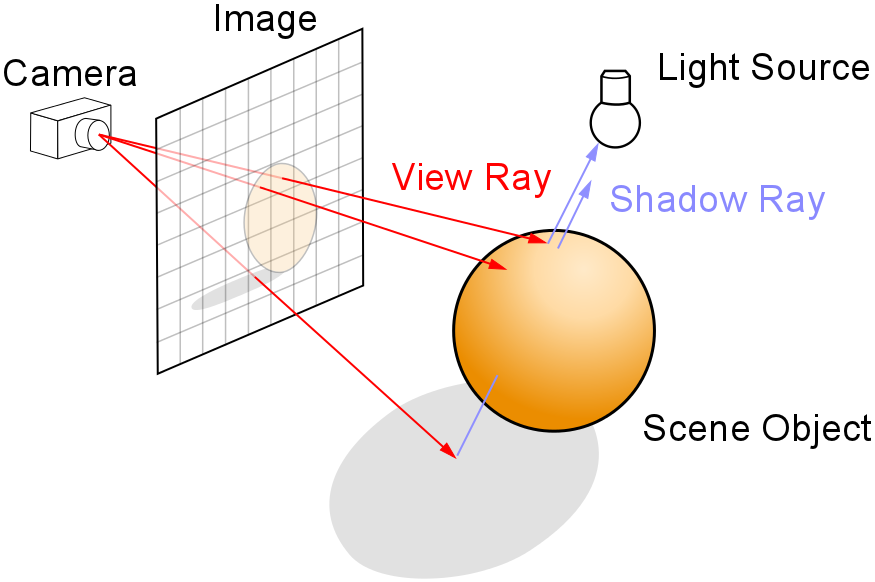
\includegraphics[width=10cm,keepaspectratio]{Ray_trace_diagram.png}
  \caption{Schéma sledování paprsků do scény, převzatý z wikipedie \cite{wikipedia}}
  \label{fig:raytrace}
\end{figure}

%%%%%%%%%%%%%%%%%%%%%%%%%%%%%%%%%%%%%%%%%%%%%%%%%%%%%%%%%%%%%%%%%%%%%%%%%%%%%%%%%%%%%%%%

\section{Popis řešení}

Jelikož Haskell je ryze funkcionální jazyk, bez použítí monád je kód velmi transparentní. Kód je rozdělen do modulů
\texttt{Math.hs}, \texttt{Phong.hs}, \texttt{Raytracer.hs}, \texttt{Scene.hs}, \texttt{Data_types.hs} a \texttt{main.hs}. 
Jádro celého algoritmu tkví ve funkci \texttt{raytracer} a \texttt{ray\_trace}. 

\begin{verbatim}
raytracer :: [Color]
raytracer = map (rt) view_grid
    where
        rt point = ray_trace get_depth 
            (Ray (vec point) camera_position point)
        vec point = normalize (point `sub` camera_position)
\end{verbatim}

Funkce \texttt{raytracer} vrhá paprsky do scény a pro výpočet výsledné barvy volá funkcí \texttt{ray\_trace}. Funkce vrací list barev,
který je předán funkci \texttt{png}, která z listu vytvoří obrázek formátu png.

\begin{verbatim}
ray_trace :: Int -> Ray -> Color 
ray_trace depth ray@(Ray vector source dest)  
    | on_ray_intersections == [] = background_color
    | otherwise = (sum_phong (apply_shade get_phong)) + reflection_color 
    where
        all_intersections = concat (map 
            (get_intersections ray) scene)
        intersections = map_filter_distance dest 
            all_intersections
        on_ray_intersections = filter 
            ((is_point_on_ray ray) . (point . snd)) 
            intersections
        closest_intersection = snd (minimum on_ray_intersections) 
        get_phong = phong closest_intersection 
            camera_position light_position
        shade = get_shade (point closest_intersection)
        apply_shade (PhongColor a d s) = 
            (PhongColor a ((fst shade) `mul_color` d) 
            ((snd shade) `mul_color` s))
        reflection_color = reflection (depth-1) closest_intersection
\end{verbatim}

Funkce \texttt{ray\_trace} bere dva parametry, hloubku raytracingu a paprsek. Vrací výslednou barvu pro daný vržený paprsek.

Procedurální textury jsou implementovány pomocí funkce \texttt{}, pro výpočet souřadnic neporcedurální textury a její namapování na objekt,
což je převod 3D souřadnice do 2D, slouží funkce \texttt{uv\_map}. Mip mapy a bilinearní filtrování jsou jako samostatný typ materiálu, stejně jako všechny
ostatní typy textur. Při výpočtu supersamplingu je ve funkci \texttt{raytrace} před funkí \texttt{ray\_trace}
volána funkce \texttt{supersample}, která paprsek nadvzorkuje, počítá průměr a v případě potřeby nadvzorkuje znovu. Je možné použít kombinace
více různých metod pro potlačení aliasu v rámci jednoho obrázku.

Implementováno byl phongův osvětlovací model, pomocí funkce se signaturou: 
\begin{verbatim}
    phong :: Intersection -> Dim3 -> Dim3 -> PhongColor 
\end{verbatim}
Jako parametry bere průsečík, pozici světla a pozici kamery, vrací barvu tohoto průsečíku.

%%%%%%%%%%%%%%%%%%%%%%%%%%%%%%%%%%%%%%%%%%%%%%%%%%%%%%%%%%%%%%%%%%%%%%%%%%%%%%%%%%%%%%%%

\section{Vyhodnocení}

supersample.png

srovnání metod 2 a 2

%%%%%%%%%%%%%%%%%%%%%%%%%%%%%%%%%%%%%%%%%%%%%%%%%%%%%%%%%%%%%%%%%%%%%%%%%%%%%%%%%%%%%%%%

\section{Závěr}

Použité metody pro potlačení aliasu jsou patrné i bez důkladného prozkoumání, zpomalení algoritmu je vzhledem k původní
době výpočtu přijatelné.

%
%
% LITERATURA
% ======================
\newpage
{%
    \renewcommand{\refname}{Literatura} % Text nadpisu thebibliography.
    \newcommand{\bi}[4]{\bibitem{#1}\textit{#2.} #3\\{}$<$\url{#4}$>$}%
    %\newcommand{\Dont}[1]{}%
    \newcommand{\citdatum}[1][2011-10-08]{$[$cit.~{#1}$]$}%
%
\begin{thebibliography}{MM}%
% Vzor: \bi{label}{Název}{Poznámky.}{http://www.adresa.cz/}%
\bi{vectoralgebra}{Vector Algebra for Ray Tracing}{\citdatum[2012-11-24]}
    {http://tom.cs.byu.edu/~455/rt.pdf}
\bi{wikipedia}{Wikipedia, The Free Encyclopedia}{\citdatum[2012-11-24]}
    {http://en.wikipedia.org/}
\end{thebibliography}}
\end{document}
